
\title{Sistemi Informativi \\ Laboratorio 4}
\author{
        Catalin Copil
            \and
        Mattia de Stefani
            \and
        Giulio Lovisotto
}
\date{\today}

\documentclass[12pt]{article}
\usepackage{algorithmicx}
\usepackage{algpseudocode}
\usepackage{graphicx}
\usepackage{geometry}

\addtolength{\topmargin}{-.5in}
\begin{document}
\maketitle

\section{Descrizione}

Visto che abbiamo scelto di usare BM25 per il ranking, applicheremo la formula tenendo in considerazione i giudizi di rilevanza. Per il relevance feedback esplicito utilizzeremo il file \texttt{qrels-treceval.txt}. Ricordiamo che la formula di BM25 tieni gia' in considerazione i giudizi di rilevanza nella sua forma base. 
\[ \sum\limits_{i \in Q}\log\Bigl(\frac{(r_i+0.5)/(R-r_i+0.5)}{(n_i-r_i+0.5)/(N-n_i-R+r_i+0.5)}\Bigl)\cdot\frac{(k_1+1)f_i}{k+f_i}\cdot\frac{(k_2+1)qf_i}{k_2+qf_i}. \]
Ricordiamo che $R$ e' il numero di documenti rilevanti per la query in questione, mentre $r_i$ e' il numero di documenti rilevanti che contiene il termine $i$.

\subsection{Relevance Feedback Esplicito}
Il reperimento avvera' in 2 step. Nel primo verra' eseguito il ranking senza informazioni di rilevanza, e tra i primi $N$ documenti verranno estratti quelli rilevanti usando il file \texttt{qrels-treceval.txt}. Poi verranno estratti i valori $R$, $r_i$ tra i documenti rilevanti individuati e verranno usati per la seconda esecuzione dell'algoritmo.

\subsection{Pseudo Relevance Feedback}
Il reperimento avvera' in 2 step. Nel primo verra' eseguito il ranking senza informazioni di rilevanza, verranno considerati i primi $N$ documenti come rilevanti. Poi verranno estratti i valori $R$, $r_i$ tra i documenti rilevanti individuati e verranno usati per la seconda esecuzione dell'algoritmo.

\section{Implementazione}
Per il calcolo di $R$ ed $r_i$, utilizzeremo la matrice che contiene la frequenza di occorrenza delle parole per ogni documento (n\_docs $\times$ n\_words). Durante il reperimento, per ogni documento, per ogni termine $i$ andremo a prendere il numero di documenti rilevanti che contiene il termine $i$, e lo salveremo in una mappa $map$ (mappa $i \rightarrow r_i$). Useremo la mappa per calcolare il ranking rispetto ai valori $R, r_i$. I documenti rilevanti sono calcolati come descritto nella precedente sezione.

\section{Risultati}
Abbiamo notato che usando il relevance feedback esplicito la precisione $map$ migliorava. Mentre utilizzando lo pseudo relevance feedback la precisione peggiorava leggermente. Figura \ref{fig:uno} mostra i risultati utilizzando la versione base di BM25 (senza giudizi di rilevanza). Figura \ref{fig:due} mostra i risultati ottenuti utilizzando feedback esplicito. Figura \ref{fig:tre} mostra i risultati ottenuti utilizzando pseudo relevance feedback.

\begin{figure}[htbp]
\begin{center}
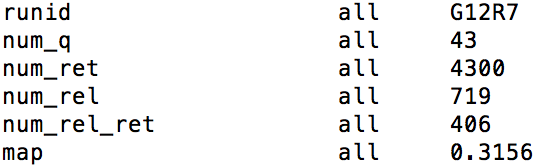
\includegraphics[width=0.75\textwidth]{base.png}
\caption{Risultati \textit{trec\_eval} BM25 base.}
\label{fig:uno}
\end{center}
\end{figure}

\begin{figure}[htbp]
\begin{center}
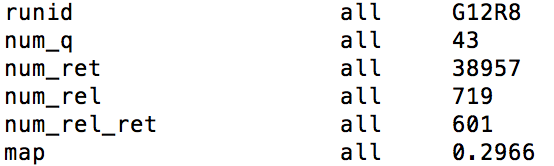
\includegraphics[width=0.75\textwidth]{pseudo.png}
\caption{Risultati \textit{trec\_eval} BM25 relevance feedback pseudo.}
\label{fig:due}
\end{center}
\end{figure}

\begin{figure}[htbp]
\begin{center}
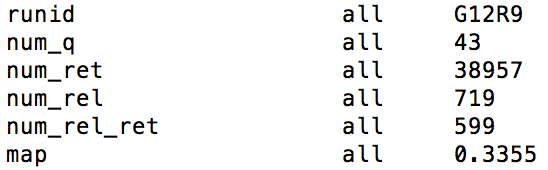
\includegraphics[width=0.75\textwidth]{esplicito.png}
\caption{Risultati \textit{trec\_eval} BM25 relevance feedback esplicito.}
\label{fig:tre}
\end{center}
\end{figure}


\bibliographystyle{abbrv}
\bibliography{main}

\end{document}